\chapter {Analyzer}

Analyzer's role is to facade objects and methods that compose this component and provide a simple interface for a processing --- analyzing --- of a single HLASM source file. The output of the analysis is data for LSP server.

\section{Overview}

\begin{figure}
	\centering
	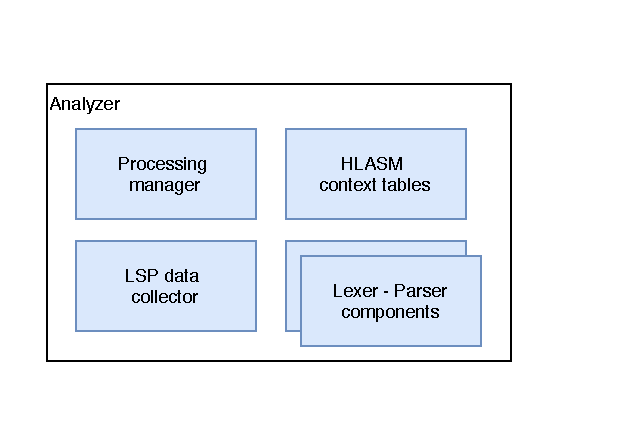
\includegraphics[width=\textwidth / 2]{img/analyzer_arch}
	\caption{The composition of Analyzer component}
	\label{fig06:analyzer}
\end{figure}

Analyzer is composed of several sub-components all required to properly process the file (see \cref{fig06:analyzer}). 
\begin{itemize}
	\item \emph{LSP data collector} collects and retieves all LSP information created while processing of the file.
	\item \emph{HLASM context tables} holds information about the context of processed HLASM source code.
	\item Analyzer facades several \emph{Lexer - Parses sub-components} to simplify the interface and ease the use of this component.
	\item \emph{Processing manager} contains the main loop where file is processed.
\end{itemize}

\subsection{Construction}

In order to parse a HLASM file, analyzer is constructed with the following parameters:
\begin{itemize}
	\item \emph{Name and content of the file}
	\item \emph{Parse library provider} -- object responsible for resolving source file dependencies. The dependencies are only discovered during the analysis, so it is not possible to provide the files beforehand.
	\item \emph{Processing tracer} (see \cref{chap:macro_tracer}).
\end{itemize}

When this constructor is used, analyzer creates HLASM context tables and analyses the provided source as an open-code. We say that analyzer has \emph{owner semantics}. 
 
Analyzer provides \emph{reference semantics} as well. The provided source is not treated as an open-code, rather as an external file dependency. The constructor of analyzer with reference semantics adds two parameters to the previous one:
\begin{itemize}
	\item \emph{HLASM context tables reference} -- belonging to the owning open-code analyzer.
	\item \emph{Library data} -- states how should be the dependency file further analyzed (see \cref{lab06:lib_data}).
\end{itemize}

This constructor is called within open-code analyzer by it's sub-components when they use Parse library provider.

\vspace{0.5cm}

To sum up, after analyzer is constructed, it analyses provided source file. In result, it updated HLASM context tables and provides a list of diagnostics linked to the file, highlighting, list of symbol definitions, etc.

\section{LSP data collector}




